\documentclass[aspectratio=169, 10pt]{beamer}

% Packages
\usepackage{fontspec}
\usepackage{hyperref}
\usepackage{graphicx}
\usepackage{tikz}
\usetikzlibrary{shapes.geometric, positioning, arrows.meta}
\usepackage{booktabs}
\usepackage{listings}
\usepackage{color}

% Font Configuration (XeLaTeX supports system fonts)
\setsansfont{Arial} % Clean, modern sans-serif font

% Custom Modern Flat Design Theme (Navy & Teal Palette)
\definecolor{primary}{RGB}{18, 30, 49}     % Dark Navy for headings
\definecolor{accent}{RGB}{0, 150, 136}      % Teal/Cyan for highlights
\definecolor{background}{RGB}{248, 249, 250} % Soft Light Gray background
\definecolor{textdark}{RGB}{33, 37, 41}     % Dark Charcoal for readable text
\definecolor{cardbg}{RGB}{255, 255, 255}    % White for card blocks

% Beamer General Styling
\setbeamercolor{background canvas}{bg=background}
\setbeamercolor{normal text}{fg=textdark}
\setbeamercolor{title}{fg=primary}
\setbeamercolor{frametitle}{fg=primary}
\setbeamercolor{structure}{fg=accent}

% Custom title page style
\setbeamerfont{title}{size=\huge, series=\bfseries}
\setbeamerfont{subtitle}{size=\large, shape=\itshape}
\setbeamerfont{frametitle}{size=\Large, series=\bfseries}

% Remove default navigation symbols
\setbeamertemplate{navigation symbols}{}

% Modern Slide Footer
\setbeamertemplate{footline}{
    \leavevmode%
    \hbox{%
        \begin{beamercolorbox}[wd=.333333\paperwidth,ht=2.25ex,dp=1ex,left]{author in head/foot}%
            \usebeamerfont{author in head/foot}\hspace*{2ex}Viettel Digital Talent 2026
        \end{beamercolorbox}%
        \begin{beamercolorbox}[wd=.333333\paperwidth,ht=2.25ex,dp=1ex,center]{title in head/foot}%
            \usebeamerfont{title in head/foot}OmniCare Presentation
        \end{beamercolorbox}%
        \begin{beamercolorbox}[wd=.333333\paperwidth,ht=2.25ex,dp=1ex,right]{date in head/foot}%
            \insertframenumber{} / \inserttotalframenumber\hspace*{2ex}
        \end{beamercolorbox}}%
    \vspace*{1ex}
}

% Card / Block styling override
\setbeamertemplate{blocks}[rounded][shadow=false]
\setbeamercolor{block title}{bg=primary!10, fg=primary}
\setbeamercolor{block body}{bg=cardbg, fg=textdark}
\setbeamercolor{block title example}{bg=accent!10, fg=accent}
\setbeamercolor{block body example}{bg=cardbg, fg=textdark}

% Presentation Information
\title{Omnichannel Customer Care System}
\subtitle{Facebook Messenger, Page Comments and Email Integration}
\author{Viettel Digital Talent 2026 - Mini Project}
\date{\today}

\begin{document}

% -------------------------------------------------------------
% SLIDE 1: Title Slide (Modern Minimalist Intro)
% -------------------------------------------------------------
\begin{frame}[plain]
    \begin{center}
        \vspace{1.5cm}
        {\color{accent}\rule{\linewidth}{1.5pt}} \\[0.4cm]
        {\usebeamerfont{title}\inserttitle} \\[0.2cm]
        {\usebeamerfont{subtitle}\insertsubtitle} \\[0.4cm]
        {\color{accent}\rule{\linewidth}{1.5pt}} \\[1cm]
        \textbf{Program:} Viettel Digital Talent 2026 \\[0.1cm]
        \textbf{Project Name:} OmniCare \\[0.1cm]
        \textbf{Topic:} Omnichannel Customer Care Workspace
    \end{center}
\end{frame}

% -------------------------------------------------------------
% SLIDE 2: Problem Statement
% -------------------------------------------------------------
\begin{frame}{Problem Statement \& Goals}
    \begin{columns}[T]
        \begin{column}{0.48\textwidth}
            \begin{block}{The Problem}
                \begin{itemize}
                    \item Customer care agents waste time switching between multiple platforms (Facebook Page, Personal Gmail).
                    \item Missing messages/comments leading to slow response times.
                    \item Lack of unified tracking, agent assignment, and audit trail.
                \end{itemize}
            \end{block}
        \end{column}
        
        \begin{column}{0.48\textwidth}
            \begin{block}{Project Goals}
                \begin{itemize}
                    \item \textbf{Consolidate}: Collect Facebook messages/comments and email into a single workspace.
                    \item \textbf{Normalize}: Standardize inbound events into a uniform model.
                    \item \textbf{Collaborate}: Support conversation assignment, state tracking, and responses.
                \end{itemize}
            \end{block}
        \end{column}
    \end{columns}
\end{frame}

% -------------------------------------------------------------
% SLIDE 3: System Architecture (C4 Context)
% -------------------------------------------------------------
\begin{frame}{System Architecture Overview}
    \begin{center}
        \begin{block}{Modular Monolith Architecture}
            System split into logical modules: \textbf{identity}, \textbf{inbox}, \textbf{facebook-adapter}, and \textbf{email-adapter}.
        \end{block}
        \vspace{0.2cm}
        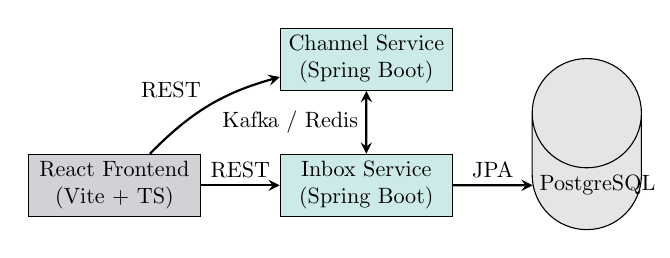
\begin{tikzpicture}[node distance=2cm, auto, >=stealth, scale=0.8, every node/.style={transform shape}]
            \node[draw, rectangle, fill=primary!20, text width=2.5cm, align=center] (client) {React Frontend\\(Vite + TS)};
            \node[draw, rectangle, fill=accent!20, text width=2.5cm, align=center, right of=client, node distance=4cm] (inbox) {Inbox Service\\(Spring Boot)};
            \node[draw, rectangle, fill=accent!20, text width=2.5cm, align=center, above of=inbox, node distance=2cm] (channel) {Channel Service\\(Spring Boot)};
            \node[draw, cylinder, fill=gray!20, text width=1.5cm, align=center, shape border rotate=90, right of=inbox, node distance=3.5cm] (db) {PostgreSQL};
            
            \path[->, thick] (client) edge node {REST} (inbox);
            \path[->, thick] (client) edge[bend left=15] node {REST} (channel);
            \path[<->, thick] (inbox) edge node {Kafka / Redis} (channel);
            \path[->, thick] (inbox) edge node {JPA} (db);
        \end{tikzpicture}
    \end{center}
\end{frame}

% -------------------------------------------------------------
% SLIDE 4: Facebook Integration - Inbound Webhooks
% -------------------------------------------------------------
\begin{frame}{Facebook Integration: Inbound Flow}
    \begin{block}{Webhook Real-time Connection}
        Facebook feeds events to the system using HTTP POST payloads with secure signatures.
    \end{block}
    \vspace{0.2cm}
    \begin{enumerate}
        \item \textbf{Handshake Verification}: Meta verification of Callback URL using the `hub.challenge` token.
        \item \textbf{Signature Validation}: Controller verifies the payload authenticity using `X-Hub-Signature-256` and the App Secret (HMAC-SHA256).
        \item \textbf{Event Extraction}:
            \begin{itemize}
                \item \textbf{Messenger}: Parses `messaging` payload for customer text inputs.
                \item \textbf{Page Comments}: Parses `feed` payload for user comments, filtering out echoes (Page's own posts/comments).
            \end{itemize}
    \end{enumerate}
\end{frame}

% -------------------------------------------------------------
% SLIDE 5: Facebook Integration - Outbound Replies
% -------------------------------------------------------------
\begin{frame}{Facebook Integration: Outbound Flow}
    \begin{block}{Graph API Communication}
        Outbound messages are pushed back to the Facebook platform programmatically.
    \end{block}
    \vspace{0.4cm}
    \begin{itemize}
        \item \textbf{Credentials}: Secured via permanent **Page Access Token** generated through Long-Lived Token Exchange.
        \item \textbf{Messenger Send API}:
            \begin{itemize}
                \item Pushes responses directly to the customer's Page Scope ID (PSID).
                \item Endpoint: `POST /v20.0/me/messages`
            \end{itemize}
        \item \textbf{Comment Reply API}:
            \begin{itemize}
                \item Posts threaded replies to specific customer comment IDs.
                \item Endpoint: `POST /v20.0/{comment-id}/comments`
            \end{itemize}
    \end{itemize}
\end{frame}

% -------------------------------------------------------------
% SLIDE 6: Email Integration - Inbound Flow
% -------------------------------------------------------------
\begin{frame}{Email Integration: Inbound Ingestion}
    \begin{block}{IMAP Polling Architecture}
        Allows asynchronous ingestion of customer emails into the Unified Inbox.
    \end{block}
    \vspace{0.2cm}
    \begin{itemize}
        \item \textbf{IMAP Protocols}: Configurable support for SSL/TLS encrypted `imaps` protocol.
        \item \textbf{State Checking}: Periodic scheduled execution loops querying target folders (e.g., `INBOX` or custom tags).
        \item \textbf{Deduplication}: Extracts `Message-ID` headers to prevent duplicate ingestion in case of repeat polls.
        \item \textbf{Formatting}: Sanitizes HTML and normalizes rich-text attachments into consistent format.
    \end{itemize}
\end{frame}

% -------------------------------------------------------------
% SLIDE 7: Email Integration - Outbound SMTP
% -------------------------------------------------------------
\begin{frame}{Email Integration: Outbound SMTP}
    \begin{block}{SMTP Reply Routing}
        Agent replies on the UI are compiled into outbound SMTP messages.
    \end{block}
    \vspace{0.3cm}
    \begin{itemize}
        \item \textbf{Mail Sender}: Integrated via Spring Boot's `JavaMailSender` abstraction.
        \item \textbf{Thread Preserving}:
            \begin{itemize}
                \item Resolves external conversation IDs to extract original `Message-ID`.
                \item Automatically sets **`In-Reply-To`** and **`References`** headers in the outgoing mail.
                \item This ensures all popular email clients (Gmail, Outlook) keep the conversation threaded correctly.
            \end{itemize}
        \item \textbf{Mocking Environment}: Uses local **Mailpit** container as a SMTP server for zero-credential offline testing.
    \end{itemize}
\end{frame}

% -------------------------------------------------------------
% SLIDE 8: Common Data Model
% -------------------------------------------------------------
\begin{frame}{Common Data Model (Normalization)}
    \begin{block}{From Platform Specifics to Domain Models}
        Decouples the business logic of the inbox from external channel schemas.
    \end{block}
    
    \begin{center}
        \begin{tabular}{lll}
            \toprule
            \textbf{Feature} & \textbf{Facebook Adapter} & \textbf{Email Adapter} \\
            \midrule
            Identity & Page Scoped ID (PSID) / Name & Email Address / Display Name \\
            Conversation & Threaded ID (`facebook:pageId:psid`) & Message-ID based hash (`email:box:id`) \\
            Payload & Message Text / Comment Media & Rich-Text Body / Attachments \\
            \bottomrule
        \end{tabular}
    \end{center}
    \vspace{0.2cm}
    All adapters map to a single domain entity: \textbf{`Conversation`} containing \textbf{`Message`} aggregates.
\end{frame}

% -------------------------------------------------------------
% SLIDE 9: Unified Inbox & Agent Workflows
% -------------------------------------------------------------
\begin{frame}{Unified Inbox \& Agent Workflows}
    \begin{columns}[T]
        \begin{column}{0.48\textwidth}
            \begin{block}{Inbox Workspace}
                \begin{itemize}
                    \item Single React UI containing active message streams.
                    \item Multi-channel filtering: select strictly `FACEBOOK` or `EMAIL` channels.
                    \item Status-based segmentation: filter threads by `OPEN`, `PENDING`, or `RESOLVED`.
                \end{itemize}
            \end{block}
        \end{column}
        
        \begin{column}{0.48\textwidth}
            \begin{block}{Agent Assignments}
                \begin{itemize}
                    \item Assign ownership of conversations to specific agents.
                    \item Live status updates (e.g. marking resolved).
                    \item Clear visual indicators for channel origin on each card.
                \end{itemize}
            \end{block}
        \end{column}
    \end{columns}
\end{frame}

% -------------------------------------------------------------
% SLIDE 10: Asynchronous Message Processing (Kafka)
% -------------------------------------------------------------
\begin{frame}{Asynchronous Event Streaming (Kafka)}
    \begin{block}{Decoupled Microservices communication}
        Ensures data consistency and decoupling between channels and inbox logic.
    \end{block}
    \vspace{0.2cm}
    \begin{center}
        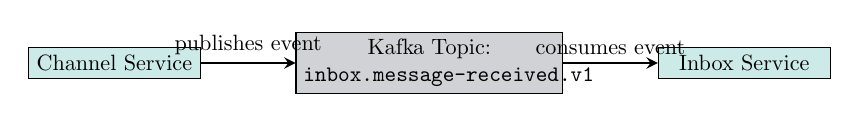
\begin{tikzpicture}[node distance=1.5cm, auto, >=stealth, scale=0.8, every node/.style={transform shape}]
            \node[draw, rectangle, fill=accent!20, text width=2.5cm, align=center] (ch) {Channel Service};
            \node[draw, rectangle, fill=primary!20, text width=4cm, align=center, right of=ch, node distance=5cm] (kafka) {Kafka Topic:\\\texttt{inbox.message-received.v1}};
            \node[draw, rectangle, fill=accent!20, text width=2.5cm, align=center, right of=kafka, node distance=5cm] (in) {Inbox Service};
            
            \path[->, thick] (ch) edge node {publishes event} (kafka);
            \path[->, thick] (kafka) edge node {consumes event} (in);
        \end{tikzpicture}
    \end{center}
    \vspace{0.2cm}
    \begin{itemize}
        \item \textbf{Resilience}: Outages in `inbox-service` will not drop incoming messages; events remain buffered in Kafka.
        \item \textbf{Retries}: Bounded exponential backoff policy for transient failures.
    \end{itemize}
\end{frame}

% -------------------------------------------------------------
% SLIDE 11: Performance & Optimization (Redis)
% -------------------------------------------------------------
\begin{frame}{Performance \& Optimization (Redis)}
    \begin{columns}[T]
        \begin{column}{0.48\textwidth}
            \begin{block}{Message Deduplication}
                \begin{itemize}
                    \item Webhook calls are not guaranteed to be delivered exactly once.
                    \item Redis stores processed `externalMessageId` with custom TTL.
                    \item Rapid duplicates are immediately discarded at the gateway level.
                \end{itemize}
            \end{block}
        \end{column}
        
        \begin{column}{0.48\textwidth}
            \begin{block}{Operational Caching}
                \begin{itemize}
                    \item Caches active configuration maps and long-lived tokens.
                    \item Decreases load on the primary PostgreSQL relational database.
                    \item Ensures fast query responses for UI inbox lists.
                \end{itemize}
            \end{block}
        \end{column}
    \end{columns}
\end{frame}

% -------------------------------------------------------------
% SLIDE 12: Demonstration & Results
% -------------------------------------------------------------
\begin{frame}{Demonstration \& Results}
    \begin{block}{Key MVP Deliverables Met}
        \begin{itemize}
            \item \textbf{E2E Flow}: Real-time Messenger messages are successfully captured and displayed.
            \item \textbf{SMTP / Mailpit}: Automated reply email threads successfully inside Mailpit client.
            \item \textbf{Robust Local Mocks}: High-coverage simulator endpoints verify E2E workflow locally without network dependencies.
        \end{itemize}
    \end{block}
    \begin{exampleblock}{Local Execution Outcome}
        All integration flows passed using local scripts (\texttt{smoke-email-flow.ps1} \& \texttt{smoke-cross-service.ps1}).
    \end{exampleblock}
\end{frame}

% -------------------------------------------------------------
% SLIDE 13: QA and Testing Strategy
% -------------------------------------------------------------
\begin{frame}{Quality Assurance \& Testing}
    \begin{block}{Multi-Layer Testing Approach}
        Ensures the stability of the monolith during local development.
    \end{block}
    \vspace{0.2cm}
    \begin{itemize}
        \item \textbf{Unit Tests}: Coverage of domain models, normalization logic, and validators.
        \item \textbf{Integration Tests}: Dockerized services running with Testcontainers (Kafka, PostgreSQL).
        \item \textbf{Automated Checks}: A unified script (\texttt{scripts/check.ps1}) compiles code, executes style checks, runs Java Maven tests (57 tests for Channel, 42 for Inbox), and builds/test the React UI.
    \end{itemize}
\end{frame}

% -------------------------------------------------------------
% SLIDE 14: Limitations & Sandbox Workarounds
% -------------------------------------------------------------
\begin{frame}{Limitations \& Sandbox Workarounds}
    \begin{block}{Development Mode Challenges}
        Meta Graph Webhooks restricts certain real events (like page feed comments) for apps in Dev Mode.
    \end{block}
    \vspace{0.2cm}
    \begin{itemize}
        \item \textbf{Limitation}: Real comments on the Page do not fire webhook events because App is not approved Live.
        \item \textbf{Solutions \& Workarounds}:
            \begin{itemize}
                \item Utilized Meta's Developer Console **Test button** to trigger fake comment payloads (verified correct handler).
                \item Configured **Dual-Mode Config Script** (\texttt{switch-mode.ps1}) to easily swap the workspace from local simulator test variables to live endpoints.
            \end{itemize}
    \end{itemize}
\end{frame}

% -------------------------------------------------------------
% SLIDE 15: Conclusion & Lessons Learned
% -------------------------------------------------------------
\begin{frame}{Conclusion \& Lessons Learned}
    \begin{block}{Key Takeaways}
        \begin{itemize}
            \item \textbf{Clean Architecture Benefit}: Adapters (Facebook, Email) are separate from core business workflows (Inbox), allowing changes in Meta APIs without breaking the inbox core.
            \item \textbf{Event Sourcing}: Designing with event-driven communication (Kafka) is critical for handling spikes in high-volume customer messages.
            \item \textbf{Testing importance}: Having deterministic mock environments (Mailpit/Simulator) speeds up development by eliminating external server delays.
        \end{itemize}
    \end{block}
    \vspace{0.4cm}
    \begin{center}
        \Large \textbf{Thank You for Your Attention! Questions?}
    \end{center}
\end{frame}

\end{document}
